\documentclass[11pt]{article}
\usepackage{fullpage}
\usepackage{algorithm}
\usepackage[noend]{algorithmic}
\usepackage{enumerate}
\usepackage{amsmath,amssymb,amsthm}
\usepackage{stackrel}
\usepackage{tikz}

% Helpful Shortcuts
\newcommand{\bc}[1]{{\quad \text{(#1)}}} 	% Justification in math env
\newcommand{\st}{{\text{ such that }}} 							   % Math env
\newcommand{\abs}[1]{{ |#1 |}} 							% Absolute value / Cardinality
\newcommand{\bld}[2]{\noindent\textbf{#1:}\hspace{0.1in}#2$  $\bigskip} % Headings
\newcommand{\notimplies}{%
	\mathrel{{\ooalign{\hidewidth$\not\phantom{=}$\hidewidth\cr$\implies$}}}}
\newcommand{\linesep}{\noindent\bigskip\rule{17cm}{0.1mm}\bigskip} % Horizontal Line
\newcommand{\Z}{\mathbb{Z}}

% These define new environments / formats for lemmas, definitions, running time, etc.
\newtheorem{lemma}{Lemma}
\newtheorem{definition}{Definition}
\newtheorem{notation}{Notation}
\newtheorem*{claim}{Claim}
\newtheorem{observation}{Observation}
\newtheorem{conjecture}[lemma]{Conjecture}
\newtheorem{theorem}[lemma]{Theorem}
\newtheorem{corollary}[lemma]{Corollary}
\newtheorem{proposition}[lemma]{Proposition}
\newtheorem*{rt}{Running Time}

% These define nice ways to format P and OPT (use \P or \opt)
\def\P{\ensuremath{$ \mathcal{P} $}}
\def\opt{\ensuremath{\textsc{opt}}}
\renewcommand{\labelenumi}{\bf \alph{enumi}.}

\renewcommand\maketitle{
	\begin{center}
		\begin{tabular*}{6.44in}{l @{\extracolsep{\fill}}c r}
			\bfseries  &  & \bfseries CSCI 383 Spring 2019 \\
			\bfseries&  & \bfseries  Module 1 Take-Home Midterm Solutions  \\
			\bfseries   &   &  \bfseries Kai Ting Keshia Yap\\ 
		\end{tabular*}
\end{center} }

\begin{document}
	\maketitle
	
	\noindent Honor Code: I affirm that I adhered to the Honor Code in this Exam. Keshia Yap
	
	\subsection*{Part 1: Closuare}
	Given a language $ A $ over the alphabet $ \{a, b\} $, we can define a new language $ Bonusa(A) $, which is any string that can be generated by taking a string from $ A $ and inserting exactly one extra $ a $ somewhere in the string. Formally: \[Bonusa(A) = \{xay \in \{a, b\}^* \mid xy\in A\}\]
	For example, $ Bonusa({ab, aba, bb}) = \{aab, aba, aaba, abaa, abb, bab, bba\} $.
	
	\begin{enumerate}
		\item Given a regular langauge $ A $, describe how to convert a DFA for $ A $ into an NFA for $ Bonusa(A) $. 
		\item Below is a DFA representing some language A. Use your procedure above to construct an NFA for $ Bonusa(A) $.
				\begin{center}
			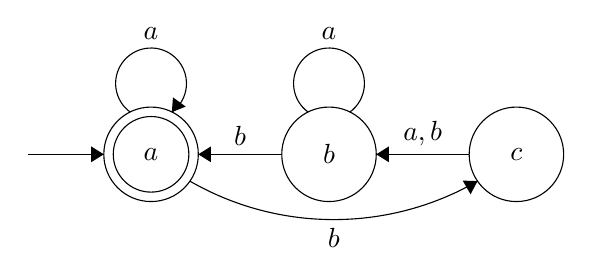
\begin{tikzpicture}[scale=0.2]
			\tikzstyle{every node}+=[inner sep=0pt]
			\draw [black] (11.5,-23.8) circle (2.4);
			\draw [black] (11.5,-23.8) circle (3);
			\draw (11.5,-23.8) node {$a$};
			\draw [black] (22.8,-23.8) circle (3);
			\draw (22.8,-23.8) node {$b$};
			\draw [black] (34.7,-23.8) circle (3);
			\draw (34.7,-23.8) node {$c$};
			\draw [black] (3.7,-23.8) -- (8.5,-23.8);
			\fill [black] (8.5,-23.8) -- (7.7,-23.3) -- (7.7,-24.3);
			\draw [black] (19.8,-23.8) -- (14.5,-23.8);
			\fill [black] (14.5,-23.8) -- (15.3,-24.3) -- (15.3,-23.3);
			\draw (17.15,-23.3) node [above] {$b$};
			\draw [black] (31.7,-23.8) -- (25.8,-23.8);
			\fill [black] (25.8,-23.8) -- (26.6,-24.3) -- (26.6,-23.3);
			\draw (28.75,-23.3) node [above] {$a,b$};
			\draw [black] (10.177,-21.12) arc (234:-54:2.25);
			\draw (11.5,-16.55) node [above] {$a$};
			\fill [black] (12.82,-21.12) -- (13.7,-20.77) -- (12.89,-20.18);
			\draw [black] (21.477,-21.12) arc (234:-54:2.25);
			\draw (22.8,-16.55) node [above] {$a$};
			\draw [black] (32.234,-25.503) arc (-60.06366:-119.93634:18.304);
			\fill [black] (32.23,-25.5) -- (31.29,-25.47) -- (31.79,-26.34);
			\draw (23.1,-28.45) node [below] {$b$};
			\end{tikzpicture}
		\end{center}
	\end{enumerate}
	\linesep
	\begin{enumerate}
		\item Given a DFA $ M=(Q,\Sigma, \delta, s,F) $ such that $ L(M)=A $, we want to construct a new DFA $ M_N $ where $ L(M_N) = Bonusa(A)$. Informally, this new DFA is comprised of two copies of the original DFA, which we will denote as $ M_1 $ and $ M_2 $. The first copy $ M_1 $ will be exactly the same as $ M $, but none of the final states of $M_N$ will be in $ M_1 $. Let $ Q':=\{q'\mid q\in Q\} $. This will be the set of states in $ M_2 $. The transition function for $ M_2 $ will be the same as in $ M $, but with the corresponding states instead. Lastly, we allow every state $M_1$ to transition to the corresponding state in $M_2$ via an $ a $.\\
		
		Formally, let $ M_N=\{Q_N, \Sigma, \Delta, S, F_N\} $, where 
		\begin{itemize}
			\item $ Q_N:=Q\cup Q' $
			\item Given that $ c\in \Sigma, c\neq a, q\in Q $, $ \Delta(q,c)=\{\delta(q,c)\} $, $ \Delta(q',c)=\{\delta(q,c)'\} $
			\item Given that $ q\in Q $, $ \Delta(q,a)=\{\delta(q,a), q'\} $
			\item $ S_N:=\{s\} $
			\item $ F_N:=\{f'\mid f\in F\} $
		\end{itemize}
		
		\item $ \\ $
		\begin{center}
			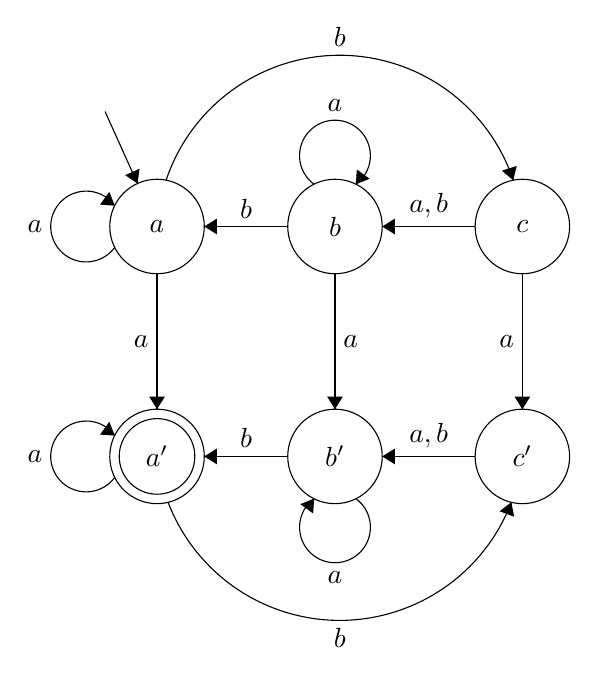
\begin{tikzpicture}[scale=0.2]
			\tikzstyle{every node}+=[inner sep=0pt]
			\draw [black] (11.5,-23.8) circle (3);
			\draw (11.5,-23.8) node {$a$};
			\draw [black] (22.8,-23.8) circle (3);
			\draw (22.8,-23.8) node {$b$};
			\draw [black] (34.7,-23.8) circle (3);
			\draw (34.7,-23.8) node {$c$};
			\draw [black] (11.5,-38.4) circle (3);
			\draw (11.5,-38.4) node {$a'$};
			\draw [black] (11.5,-38.4) circle (2.4);
			\draw [black] (22.8,-38.4) circle (3);
			\draw (22.8,-38.4) node {$b'$};
			\draw [black] (34.7,-38.4) circle (3);
			\draw (34.7,-38.4) node {$c'$};
			\draw [black] (8.2,-16.5) -- (10.26,-21.07);
			\fill [black] (10.26,-21.07) -- (10.39,-20.13) -- (9.48,-20.54);
			\draw [black] (19.8,-23.8) -- (14.5,-23.8);
			\fill [black] (14.5,-23.8) -- (15.3,-24.3) -- (15.3,-23.3);
			\draw (17.15,-23.3) node [above] {$b$};
			\draw [black] (31.7,-23.8) -- (25.8,-23.8);
			\fill [black] (25.8,-23.8) -- (26.6,-24.3) -- (26.6,-23.3);
			\draw (28.75,-23.3) node [above] {$a,b$};
			\draw [black] (8.82,-25.123) arc (-36:-324:2.25);
			\draw (4.25,-23.8) node [left] {$a$};
			\fill [black] (8.82,-22.48) -- (8.47,-21.6) -- (7.88,-22.41);
			\draw [black] (21.477,-21.12) arc (234:-54:2.25);
			\draw (22.8,-16.55) node [above] {$a$};
			\fill [black] (24.12,-21.12) -- (25,-20.77) -- (24.19,-20.18);
			\draw [black] (19.8,-38.4) -- (14.5,-38.4);
			\fill [black] (14.5,-38.4) -- (15.3,-38.9) -- (15.3,-37.9);
			\draw (17.15,-37.9) node [above] {$b$};
			\draw [black] (31.7,-38.4) -- (25.8,-38.4);
			\fill [black] (25.8,-38.4) -- (26.6,-38.9) -- (26.6,-37.9);
			\draw (28.75,-37.9) node [above] {$a,b$};
			\draw [black] (8.82,-39.723) arc (324:36:2.25);
			\draw (4.25,-38.4) node [left] {$a$};
			\fill [black] (8.82,-37.08) -- (8.47,-36.2) -- (7.88,-37.01);
			\draw [black] (24.123,-41.08) arc (54:-234:2.25);
			\draw (22.8,-45.65) node [below] {$a$};
			\fill [black] (21.48,-41.08) -- (20.6,-41.43) -- (21.41,-42.02);
			\draw [black] (34.7,-26.8) -- (34.7,-35.4);
			\fill [black] (34.7,-35.4) -- (35.2,-34.6) -- (34.2,-34.6);
			\draw (34.2,-31.1) node [left] {$a$};
			\draw [black] (22.8,-26.8) -- (22.8,-35.4);
			\fill [black] (22.8,-35.4) -- (23.3,-34.6) -- (22.3,-34.6);
			\draw (23.3,-31.1) node [right] {$a$};
			\draw [black] (11.5,-26.8) -- (11.5,-35.4);
			\fill [black] (11.5,-35.4) -- (12,-34.6) -- (11,-34.6);
			\draw (11,-31.1) node [left] {$a$};
			\draw [black] (12.076,-20.864) arc (161.50227:18.49773:11.624);
			\fill [black] (34.12,-20.86) -- (34.34,-19.95) -- (33.4,-20.26);
			\draw (23.1,-12.43) node [above] {$b$};
			\draw [black] (33.999,-41.308) arc (-20.9172:-159.0828:11.668);
			\fill [black] (34,-41.31) -- (33.25,-41.88) -- (34.18,-42.23);
			\draw (23.1,-49.31) node [below] {$b$};
			\end{tikzpicture}
		\end{center}
	\end{enumerate}

    \newpage
	\subsection*{Part 2: Pumping Lemma}
	Using the pumping lemma, prove that each of the two languages below are not regular.
	\begin{enumerate}
		\item $ L_1=\{xx\mid x\in \{0,1\}^*\} $
		\item $ L_2=\{a^{n^3}\mid n\geq 0\} $
	\end{enumerate}
	\linesep
	\begin{enumerate}
		\item \begin{proof}
		Suppose, by way of contradiction that there exists some DFA $ M_1 $ such that $ L(M_1)=L_1$, and $ F $ is the set of final states of $ M_1 $. Without loss of generality, suppose this DFA has $ k $ states. Then by definition of $ L_1 $, the string $ x_1x_2\dots x_k x_1x_2\dots x_k\in L_1 $, where $x_i\in \Sigma$, $\forall i\in[1,k]$. By the pigeon-hole principle, there exists two distinct integers $ 0\leq i<j\leq k $ such that $ \hat{\delta}(s, x_1x_2\dots x_i)=\hat{\delta}(s, x_1x_2\dots x_j) $ where $ x_1x_2\dots x_i $ is defined to be $ \varepsilon $ if $ i=0 $. Let $ u= x_1x_2\dots x_i, v=x_{i+1}x_{i+2}\dots x_j, w=x_{j+1}x_{j+2}\dots x_k, z=x_1x_2\dots x_k$; so $ uvwz\in L_1$. Then  
		\begin{align*}
			\hat{\delta}(s, u)&=\hat{\delta}(s,uv)&&\bc{by substitution}\\
			\hat{\delta}(s,uwz)&=\hat{\delta}(\hat{\delta}(s,u),wz)&&\bc{def of $ \hat{\delta} $}\\
			&=\hat{\delta}(\hat{\delta}(s,uv),wz)&&\bc{from above}\\
			&=\hat{\delta}(s,uvwz)&&\bc{def of $ \hat{\delta} $}\\
			&=\hat{\delta}(s,x_1x_2\dots x_k x_1x_2\dots x_k)&&\bc{by substitution}\\
			&\in F&&\bc{def of $L_1$}
		\end{align*}
		So $ uwz= x_1x_2\dots x_i x_{j+1}x_{j+2}\dots x_k x_1x_2\dots x_k\in L_1$. However, since the $ x_i $'s were arbitrary, we can choose $ x_1= 0$, $ x_\ell=1 $ for all $ 2\leq \ell\leq k $. Then $ uwz=01^{k-(j-i)}01^k $ which is not in $ L_1 $ since $ i<j\implies k-(j-i)<k \implies 01^{k-(j-i)}\neq01^k $. So $ L(M_1)\neq L_1 $. Contradiction.
		\end{proof}
		
		\item \begin{proof}
		Suppose, by way of contradiction that there exists some DFA $ M_2 $ such that $ L(M_2)=L_2 $, and $ F $ is the set of final states of $ M_2 $. Without loss of generality, suppose this DFA has $ k $ states. Then by definition of $ L_2 $, the string $ a^{k^3}\in L_2 $. By the pigeon-hole principle, there exists two distinct integers $ 0\leq i<j\leq k $ such that $ \hat{\delta}(s, a^i)=\hat{\delta}(s,a^j) $ where $ a^0=\varepsilon $. Let $ u= a^i, v=a^{j-i}, w=a^{k-j}, z=a^{k^3-k}$; so $ uvwz=a^{k^3}\in L_1$. Then  
		\begin{align*}
		 \hat{\delta}(s, u)&=\hat{\delta}(s,uv)&&\bc{by substitution}\\
		\hat{\delta}(s,uv^2wz)&=\hat{\delta}(\hat{\delta}(s,uv),vwz)&&\bc{def of $ \hat{\delta} $}\\
		&=\hat{\delta}(\hat{\delta}(s,u),vwz)&&\bc{from above}\\
		&=\hat{\delta}(s,uvwz)&&\bc{def of $ \hat{\delta} $}\\
		&=\hat{\delta}(s,a^{k^3})&&\bc{substitution}\\
		&\in F&&\bc{def of $L_2$}\\
		\implies uv^2wz&\in L_2	\\
		\abs{uv^2wz}&=\abs{u}+\abs{v^2}+\abs{w}+\abs{z}\\
		&=\abs{v}+(\abs{u}+\abs{v}+\abs{w}+\abs{z})\\
		&=(j-i)+k^3\\
		&\leq k+k^3\\
		&\leq k^3+3k^2+3k+1\\
		&<(k+1)^3
		\end{align*}
	\end{proof}
		
		So $ (j-i)+k^3\neq \ell^3 $ for all integers $ \ell $. Therefore, $ L(M_2)\neq L_2 $. Contradiction. \bigskip
	\end{enumerate}
	
	\newpage
	\subsection*{Part 3: True or False}
	For each of the following statements, prove the statement or disprove it with a counterexample.
	Counterexamples should be well-explained.
	\begin{enumerate}
		\item For any languages $ A,B\subseteq \Sigma^* $, if $ A $ is not regular and $ A \subseteq B $, then $ B $ is not regular.
		\item For any languages $ A,B\subseteq \Sigma ^*$, if neither $ A $ nor $ B $ are regular, then neither is $ A \cap B $.
		\item For any language $ A \subseteq \Sigma^* $, if A is not regular, then neither is $ \sim A. $
		\item No infinite subset of $ \{a^nb^n\mid n\geq 0\} $ is regular.
	\end{enumerate}
	\linesep
	\begin{enumerate}
		\item False; consider $ A=\{a^nb^n\mid n\geq 0 \} $, $ B=\{a^nb^m\mid m,n\geq 0 \} $. Clearly $ A\subseteq B $, but we proved in class that $ A $ is not regular but $ B $ is regular. 
		\item False; consider $ A=\{a^nb^n\mid n\geq 0 \} $, $ B=\{b^na^n\mid n\geq 0 \} $. Clearly $ A\cap B=\{\} $. We proved in class that $ A $ is not regular. Since non-regular languages are closed under character substitution, $ B $ is non-regular as it is simply $ A $ with the substitution $ a\mapsto b, b\mapsto a $. However the empty language is regular. 
		\item True. \textit{Proof. } We first claim that $ \sim (\sim A)=A $. This is because $\sim (\sim A)=\Sigma^*-(\Sigma^*-A)=A$. \\
		
		Now, suppose by way of contradiction, that $ \sim A $ is regular. Then since regular languages are closed under $ \sim  $ as shown in class, $ \sim (\sim A)=A $ is regular, contradicting the assumption that $ A $ is not regular. \qed
		\item True. \textit{Proof. }First, let $ B $ be any infinite subset of $ \{a^nb^n\mid n\geq 0\}  $. We claim that for any non-negative $ k $, there exists some positive integer $ m $ such that $ m\geq k $ such that $ a^mb^m\in B $. Suppose not, by way of contradiction. Then there exists some integer $ N $ such that $ B\subseteq \{a^nb^n\mid 0\leq n\leq N\} $, which is has $ N+1 $ items and is finite, so $ B $ is finite. Contradiction. \\
		
		Now, suppose that there exists an infinite subset $ B' $ of $ \{a^nb^n\mid n\geq 0\}  $ that is regular. That is, there exists a DFA $ M' $ such that $ L(M')=B' $. Then this DFA has some $ k'\in\Z $ states. By our claim, there exists some integer $ N' $ such that $ k'\leq N' $, and $ a^{N'}b^{N'} \in B'$. \\
		
		We shall now use the pumping lemma to show that $ M' $ cannot be regular. Let $ x=\varepsilon, y=a^k, z=a^{N'-k}b^{N'} $; so $  a^{N'}b^{N'}=xyz $. By the pigeon-hole principle, there exists two distinct integers $ 0\leq i<j\leq k $ such that $ \hat{\delta}(s, a^i)=\hat{\delta}(s, a^j) $. Let $ u= a^i, v=a^{j-i}, w=a^{k-j}$; so $ y=uvw $. Then  
		
		\begin{align*}
		\hat{\delta}(s, u)&=\hat{\delta}(s,uv)&&\bc{by substitution}\\
		 \hat{\delta}(s,uwz)&=\hat{\delta}(\hat{\delta}(s,u)wz) &&\bc{def of $ \hat{\delta} $}\\
		 &=\hat{\delta}(\hat{\delta}(s,uv)wz) &&\bc{from above}\\
		 &=\hat{\delta}(s,uvwz) &&\bc{def of $ \hat{\delta} $}\\
		 &=\hat{\delta}(\delta(s,x),uvwz) &&\bc{since $ \delta(s,x) =\delta(s,\varepsilon)=s$}\\
		 &=\hat{\delta}(s,xuvwz) &&\bc{def of $ \hat{\delta} $}\\
		 &=\hat{\delta}(s, a^{N'}b^{N'}) &&\bc{def of $x,u,v,w,z$}\\
		 &\in F&&\bc{def of $ N' $}
		\end{align*}
		
		This implies that $ uwz\in B'$. However, $ uwz=a^{N'-(j-i)}b^{N'} $, but clearly since $ i<j $, $ N'-(j-i)\neq N' $, so $ uwz\not\in \{a^nb^n\mid n\geq 0\} $, contradicting the assumption that $ B'\subseteq \{a^nb^n\mid n\geq 0\} $. \qed \bigskip
	\end{enumerate}

	\subsection*{Part 4: Regular Expressions}
%	Give a regular expression for each of the following languages. If it is not obvious that the expression
%	is correct, you should provide some explanation.
	\begin{enumerate}
		\item $ L_3=\{x\in \{a,b\}^*\mid \#a(x)\geq 2, \#b(x)\geq 1\} $
		\item $ L_4=\{x\in\{a,b\}^*\mid x $ does not does not contain the contiguous substring $ ab\} $
		\item $ L_5=\sim \{a^l b^m c^n\mid l,m,n\geq 0\} $
	\end{enumerate}
	\linesep
	\begin{enumerate}
		\item $ (a+b)^* (bab^*a+ab^*ab+abb^*a)(a+b)^*$
		\item $ b^*a^* $
		\item $ (a+b+c)^*(ba+ca+cb)(a+b+c)^* $
	\end{enumerate}
\end{document}